\documentclass{standalone}
\usepackage{tikz}
\usetikzlibrary{patterns, positioning}

\begin{document}
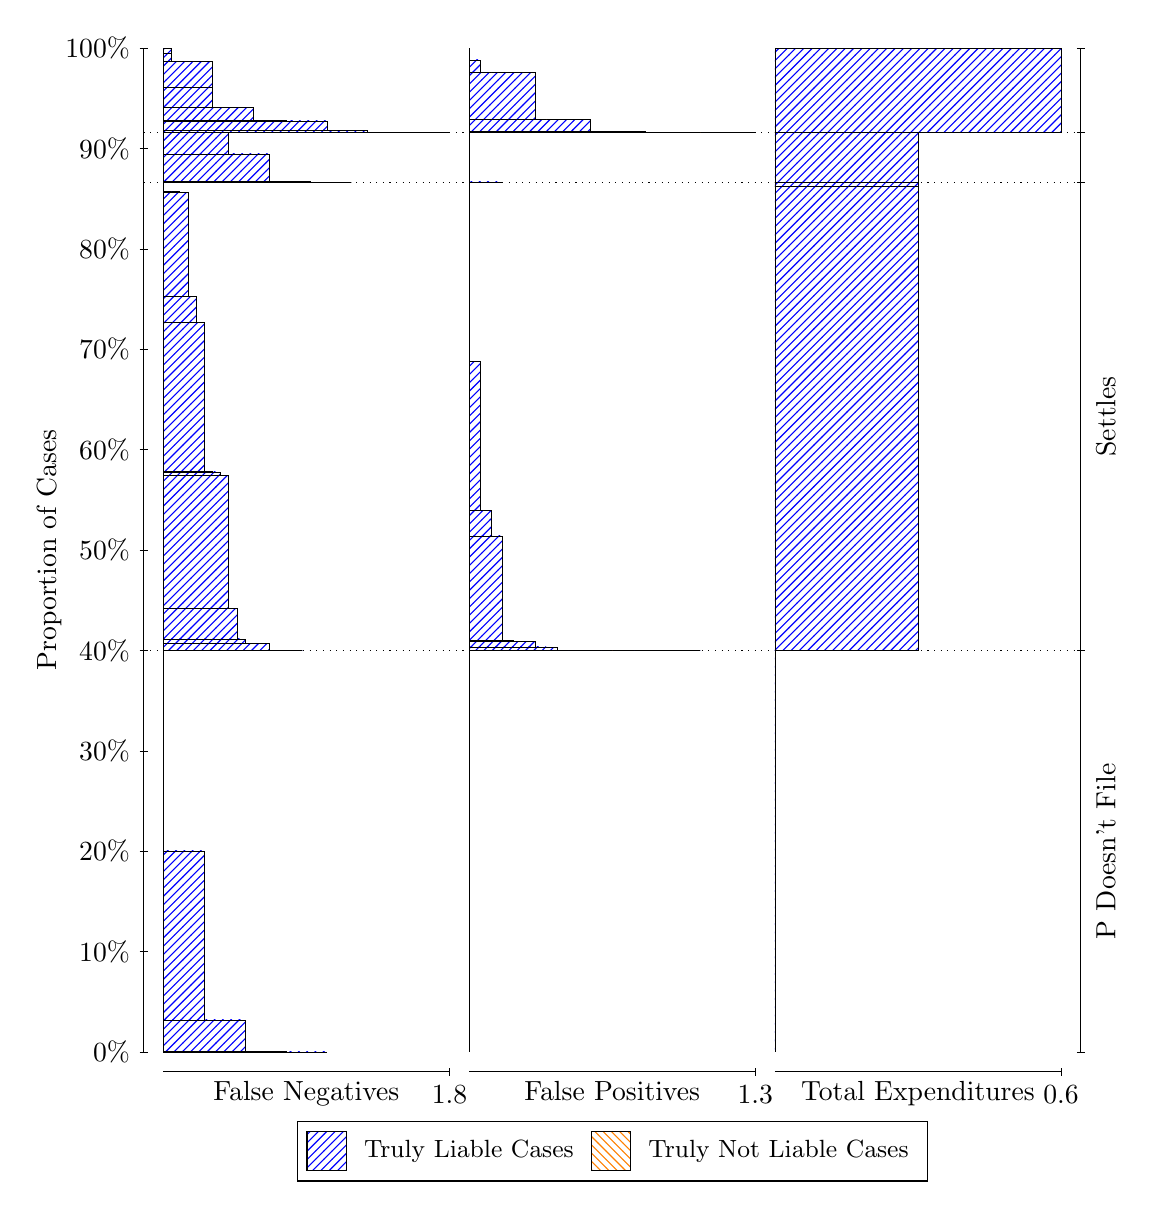
\begin{tikzpicture}
\draw[black, very thin] (1.5,1.75) -- (1.5,14.5);
\node[rotate=90, anchor=center] at (0.3, 8.125) {Proportion of Cases};
\draw[black, very thin] (1.45,1.75) -- (1.55,1.75);
\node[anchor=east] at (1.45, 1.75) {0\%};
\draw[black, very thin] (1.45,3.025) -- (1.55,3.025);
\node[anchor=east] at (1.45, 3.025) {10\%};
\draw[black, very thin] (1.45,4.3) -- (1.55,4.3);
\node[anchor=east] at (1.45, 4.3) {20\%};
\draw[black, very thin] (1.45,5.575) -- (1.55,5.575);
\node[anchor=east] at (1.45, 5.575) {30\%};
\draw[black, very thin] (1.45,6.85) -- (1.55,6.85);
\node[anchor=east] at (1.45, 6.85) {40\%};
\draw[black, very thin] (1.45,8.125) -- (1.55,8.125);
\node[anchor=east] at (1.45, 8.125) {50\%};
\draw[black, very thin] (1.45,9.4) -- (1.55,9.4);
\node[anchor=east] at (1.45, 9.4) {60\%};
\draw[black, very thin] (1.45,10.675) -- (1.55,10.675);
\node[anchor=east] at (1.45, 10.675) {70\%};
\draw[black, very thin] (1.45,11.95) -- (1.55,11.95);
\node[anchor=east] at (1.45, 11.95) {80\%};
\draw[black, very thin] (1.45,13.225) -- (1.55,13.225);
\node[anchor=east] at (1.45, 13.225) {90\%};
\draw[black, very thin] (1.45,14.5) -- (1.55,14.5);
\node[anchor=east] at (1.45, 14.5) {100\%};

\draw[black, very thin] (13.4,1.75) -- (13.4,14.5);
\draw[black, very thin] (13.35,1.75) -- (13.45,1.75);
\node[anchor=west] at (13.35, 1.75) {};
\draw[black, very thin] (13.35,6.8489) -- (13.45,6.8489);
\node[anchor=west] at (13.35, 6.8489) {};
\draw[black, very thin] (13.35,12.796) -- (13.45,12.796);
\node[anchor=west] at (13.35, 12.796) {};
\draw[black, very thin] (13.35,13.431) -- (13.45,13.431);
\node[anchor=west] at (13.35, 13.431) {};
\draw[black, very thin] (13.35,14.5) -- (13.45,14.5);
\node[anchor=west] at (13.35, 14.5) {};

\draw[black, very thin, pattern color=blue, pattern=north east lines] (1.75,1.75) rectangle (3.8262,1.75);
\draw[black, very thin, pattern color=blue, pattern=north east lines] (1.75,1.75) rectangle (3.3071,1.7534);
\draw[black, very thin, pattern color=blue, pattern=north east lines] (1.75,1.7534) rectangle (2.7881,2.158);
\draw[black, very thin, pattern color=blue, pattern=north east lines] (1.75,2.158) rectangle (2.269,4.3029);
\draw[black, very thin, pattern color=orange, pattern=north west lines] (1.75,4.3029) rectangle (1.75,4.3029);
\draw[black, very thin, pattern color=blue, pattern=north east lines] (1.75,4.3029) rectangle (1.75,6.8489);
\draw[black, very thin, pattern color=blue, pattern=north east lines] (1.75,6.8489) rectangle (3.5148,6.8489);
\draw[black, very thin, pattern color=blue, pattern=north east lines] (1.75,6.8489) rectangle (3.3071,6.849);
\draw[black, very thin, pattern color=blue, pattern=north east lines] (1.75,6.849) rectangle (3.0995,6.9394);
\draw[black, very thin, pattern color=blue, pattern=north east lines] (1.75,6.9394) rectangle (2.9957,6.9413);
\draw[black, very thin, pattern color=blue, pattern=north east lines] (1.75,6.9413) rectangle (2.8919,6.9418);
\draw[black, very thin, pattern color=blue, pattern=north east lines] (1.75,6.9418) rectangle (2.7881,6.9964);
\draw[black, very thin, pattern color=blue, pattern=north east lines] (1.75,6.9964) rectangle (2.6843,7.386);
\draw[black, very thin, pattern color=blue, pattern=north east lines] (1.75,7.386) rectangle (2.5805,9.0749);
\draw[black, very thin, pattern color=blue, pattern=north east lines] (1.75,9.0749) rectangle (2.4767,9.1159);
\draw[black, very thin, pattern color=blue, pattern=north east lines] (1.75,9.1159) rectangle (2.3729,9.1265);
\draw[black, very thin, pattern color=blue, pattern=north east lines] (1.75,9.1265) rectangle (2.269,11.014);
\draw[black, very thin, pattern color=blue, pattern=north east lines] (1.75,11.014) rectangle (2.1652,11.341);
\draw[black, very thin, pattern color=blue, pattern=north east lines] (1.75,11.341) rectangle (2.0614,12.669);
\draw[black, very thin, pattern color=blue, pattern=north east lines] (1.75,12.669) rectangle (1.9576,12.677);
\draw[black, very thin, pattern color=blue, pattern=north east lines] (1.75,12.677) rectangle (1.8538,12.677);
\draw[black, very thin, pattern color=orange, pattern=north west lines] (1.75,12.677) rectangle (1.75,12.677);
\draw[black, very thin, pattern color=blue, pattern=north east lines] (1.75,12.677) rectangle (1.75,12.796);
\draw[black, very thin, pattern color=blue, pattern=north east lines] (1.75,12.796) rectangle (4.1376,12.796);
\draw[black, very thin, pattern color=blue, pattern=north east lines] (1.75,12.796) rectangle (3.6186,12.804);
\draw[black, very thin, pattern color=blue, pattern=north east lines] (1.75,12.804) rectangle (3.0995,13.155);
\draw[black, very thin, pattern color=blue, pattern=north east lines] (1.75,13.155) rectangle (2.5805,13.428);
\draw[black, very thin, pattern color=blue, pattern=north east lines] (1.75,13.428) rectangle (2.0614,13.431);
\draw[black, very thin, pattern color=orange, pattern=north west lines] (1.75,13.431) rectangle (1.75,13.431);
\draw[black, very thin, pattern color=blue, pattern=north east lines] (1.75,13.431) rectangle (5.3833,13.431);
\draw[black, very thin, pattern color=blue, pattern=north east lines] (1.75,13.431) rectangle (4.8643,13.431);
\draw[black, very thin, pattern color=blue, pattern=north east lines] (1.75,13.431) rectangle (4.3452,13.457);
\draw[black, very thin, pattern color=blue, pattern=north east lines] (1.75,13.457) rectangle (3.93,13.457);
\draw[black, very thin, pattern color=blue, pattern=north east lines] (1.75,13.457) rectangle (3.8262,13.575);
\draw[black, very thin, pattern color=blue, pattern=north east lines] (1.75,13.575) rectangle (3.411,13.575);
\draw[black, very thin, pattern color=blue, pattern=north east lines] (1.75,13.575) rectangle (3.3071,13.582);
\draw[black, very thin, pattern color=blue, pattern=north east lines] (1.75,13.582) rectangle (2.8919,13.742);
\draw[black, very thin, pattern color=blue, pattern=north east lines] (1.75,13.742) rectangle (2.7881,13.742);
\draw[black, very thin, pattern color=blue, pattern=north east lines] (1.75,13.742) rectangle (2.3729,14);
\draw[black, very thin, pattern color=blue, pattern=north east lines] (1.75,14) rectangle (2.3729,14.335);
\draw[black, very thin, pattern color=blue, pattern=north east lines] (1.75,14.335) rectangle (2.269,14.335);
\draw[black, very thin, pattern color=blue, pattern=north east lines] (1.75,14.335) rectangle (1.8538,14.427);
\draw[black, very thin, pattern color=blue, pattern=north east lines] (1.75,14.427) rectangle (1.8538,14.494);
\draw[black, very thin, pattern color=orange, pattern=north west lines] (1.75,14.494) rectangle (1.75,14.494);
\draw[black, very thin, pattern color=blue, pattern=north east lines] (1.75,14.494) rectangle (1.75,14.5);
\draw[black, very thin, pattern color=orange, pattern=north west lines] (5.6333,1.75) rectangle (5.6333,1.75);
\draw[black, very thin, pattern color=blue, pattern=north east lines] (5.6333,1.75) rectangle (5.6333,6.8489);
\draw[black, very thin, pattern color=orange, pattern=north west lines] (5.6333,6.8489) rectangle (8.5679,6.8489);
\draw[black, very thin, pattern color=blue, pattern=north east lines] (5.6333,6.8489) rectangle (8.5679,6.8489);
\draw[black, very thin, pattern color=orange, pattern=north west lines] (5.6333,6.8489) rectangle (8.009,6.8489);
\draw[black, very thin, pattern color=blue, pattern=north east lines] (5.6333,6.8489) rectangle (8.009,6.8489);
\draw[black, very thin, pattern color=blue, pattern=north east lines] (5.6333,6.8489) rectangle (7.8692,6.8489);
\draw[black, very thin, pattern color=orange, pattern=north west lines] (5.6333,6.8489) rectangle (7.7295,6.8489);
\draw[black, very thin, pattern color=blue, pattern=north east lines] (5.6333,6.8489) rectangle (7.7295,6.8489);
\draw[black, very thin, pattern color=orange, pattern=north west lines] (5.6333,6.8489) rectangle (7.45,6.8489);
\draw[black, very thin, pattern color=blue, pattern=north east lines] (5.6333,6.8489) rectangle (7.45,6.8489);
\draw[black, very thin, pattern color=blue, pattern=north east lines] (5.6333,6.8489) rectangle (7.3103,6.8489);
\draw[black, very thin, pattern color=orange, pattern=north west lines] (5.6333,6.8489) rectangle (7.1705,6.8489);
\draw[black, very thin, pattern color=blue, pattern=north east lines] (5.6333,6.8489) rectangle (7.1705,6.8489);
\draw[black, very thin, pattern color=blue, pattern=north east lines] (5.6333,6.8489) rectangle (7.0308,6.8489);
\draw[black, very thin, pattern color=orange, pattern=north west lines] (5.6333,6.8489) rectangle (6.891,6.8489);
\draw[black, very thin, pattern color=blue, pattern=north east lines] (5.6333,6.8489) rectangle (6.891,6.8489);
\draw[black, very thin, pattern color=blue, pattern=north east lines] (5.6333,6.8489) rectangle (6.7513,6.893);
\draw[black, very thin, pattern color=blue, pattern=north east lines] (5.6333,6.893) rectangle (6.6115,6.8955);
\draw[black, very thin, pattern color=blue, pattern=north east lines] (5.6333,6.8955) rectangle (6.4718,6.9675);
\draw[black, very thin, pattern color=blue, pattern=north east lines] (5.6333,6.9675) rectangle (6.3321,6.9679);
\draw[black, very thin, pattern color=blue, pattern=north east lines] (5.6333,6.9679) rectangle (6.1923,6.9756);
\draw[black, very thin, pattern color=blue, pattern=north east lines] (5.6333,6.9756) rectangle (6.0526,8.3035);
\draw[black, very thin, pattern color=blue, pattern=north east lines] (5.6333,8.3035) rectangle (5.9128,8.6308);
\draw[black, very thin, pattern color=blue, pattern=north east lines] (5.6333,8.6308) rectangle (5.7731,10.518);
\draw[black, very thin, pattern color=blue, pattern=north east lines] (5.6333,10.518) rectangle (5.6333,12.796);
\draw[black, very thin, pattern color=orange, pattern=north west lines] (5.6333,12.796) rectangle (6.0526,12.796);
\draw[black, very thin, pattern color=blue, pattern=north east lines] (5.6333,12.796) rectangle (6.0526,12.799);
\draw[black, very thin, pattern color=blue, pattern=north east lines] (5.6333,12.799) rectangle (5.6333,13.431);
\draw[black, very thin, pattern color=orange, pattern=north west lines] (5.6333,13.431) rectangle (9.2667,13.431);
\draw[black, very thin, pattern color=blue, pattern=north east lines] (5.6333,13.431) rectangle (9.2667,13.431);
\draw[black, very thin, pattern color=orange, pattern=north west lines] (5.6333,13.431) rectangle (8.5679,13.431);
\draw[black, very thin, pattern color=blue, pattern=north east lines] (5.6333,13.431) rectangle (8.5679,13.431);
\draw[black, very thin, pattern color=orange, pattern=north west lines] (5.6333,13.431) rectangle (7.8692,13.431);
\draw[black, very thin, pattern color=blue, pattern=north east lines] (5.6333,13.431) rectangle (7.8692,13.437);
\draw[black, very thin, pattern color=orange, pattern=north west lines] (5.6333,13.437) rectangle (7.1705,13.437);
\draw[black, very thin, pattern color=blue, pattern=north east lines] (5.6333,13.437) rectangle (7.1705,13.596);
\draw[black, very thin, pattern color=orange, pattern=north west lines] (5.6333,13.596) rectangle (6.6115,13.596);
\draw[black, very thin, pattern color=blue, pattern=north east lines] (5.6333,13.596) rectangle (6.6115,13.596);
\draw[black, very thin, pattern color=blue, pattern=north east lines] (5.6333,13.596) rectangle (6.4718,14.189);
\draw[black, very thin, pattern color=orange, pattern=north west lines] (5.6333,14.189) rectangle (5.9128,14.189);
\draw[black, very thin, pattern color=blue, pattern=north east lines] (5.6333,14.189) rectangle (5.9128,14.189);
\draw[black, very thin, pattern color=blue, pattern=north east lines] (5.6333,14.189) rectangle (5.7731,14.349);
\draw[black, very thin, pattern color=orange, pattern=north west lines] (5.6333,14.349) rectangle (5.6333,14.349);
\draw[black, very thin, pattern color=blue, pattern=north east lines] (5.6333,14.349) rectangle (5.6333,14.5);
\draw[black, very thin, pattern color=orange, pattern=north west lines] (9.5167,1.75) rectangle (9.5167,1.75);
\draw[black, very thin, pattern color=blue, pattern=north east lines] (9.5167,1.75) rectangle (9.5167,6.8489);
\draw[black, very thin, pattern color=orange, pattern=north west lines] (9.5167,6.8489) rectangle (11.333,6.8489);
\draw[black, very thin, pattern color=blue, pattern=north east lines] (9.5167,6.8489) rectangle (11.333,12.745);
\draw[black, very thin, pattern color=orange, pattern=north west lines] (9.5167,12.745) rectangle (11.333,12.745);
\draw[black, very thin, pattern color=blue, pattern=north east lines] (9.5167,12.745) rectangle (11.333,12.796);
\draw[black, very thin, pattern color=orange, pattern=north west lines] (9.5167,12.796) rectangle (11.333,12.796);
\draw[black, very thin, pattern color=blue, pattern=north east lines] (9.5167,12.796) rectangle (11.333,13.431);
\draw[black, very thin, pattern color=orange, pattern=north west lines] (9.5167,13.431) rectangle (13.15,13.431);
\draw[black, very thin, pattern color=blue, pattern=north east lines] (9.5167,13.431) rectangle (13.15,14.5);
\draw[black, dotted] (1.5,6.8489) -- (13.4,6.8489);
\draw[black, dotted] (1.5,12.796) -- (13.4,12.796);
\draw[black, dotted] (1.5,13.431) -- (13.4,13.431);
\draw[black, very thin] (1.75,1.5) -- (5.3833,1.5);
\node[anchor=north] at (3.5667, 1.5) {False Negatives};
\draw[black, very thin] (5.3833,1.45) -- (5.3833,1.55);
\node[anchor=north] at (5.3833, 1.45) {1.8};

\draw[black, very thin] (5.6333,1.5) -- (9.2667,1.5);
\node[anchor=north] at (7.45, 1.5) {False Positives};
\draw[black, very thin] (9.2667,1.45) -- (9.2667,1.55);
\node[anchor=north] at (9.2667, 1.45) {1.3};

\draw[black, very thin] (9.5167,1.5) -- (13.15,1.5);
\node[anchor=north] at (11.333, 1.5) {Total Expenditures};
\draw[black, very thin] (13.15,1.45) -- (13.15,1.55);
\node[anchor=north] at (13.15, 1.45) {0.6};

\node[black, centered, rotate=90] at (13.72, 4.2994) {P Doesn't File};
\node[black, centered, rotate=90] at (13.72, 9.8224) {Settles};



\draw (7.449999999999999,1.5) node[draw=none] (baseCoordinate) {};
\begin{scope}[align=center]
        \matrix[scale=0.5, draw=black, below=0.5cm of baseCoordinate, nodes={draw}, column sep=0.1cm]{
            \node[rectangle, draw, minimum width=0.5cm, minimum height=0.5cm, pattern=north east lines, pattern color=blue] {}; &
            \node[draw=none, font=\small] (B) {Truly Liable Cases}; &
            \node[rectangle, draw, minimum width=0.5cm, minimum height=0.5cm, pattern=north west lines, pattern color=orange] {}; &
            \node[draw=none, font=\small] (B) {Truly Not Liable Cases}; \\
            };
\end{scope}

\end{tikzpicture}
\end{document}